\documentclass[a4j,10pt]{jarticle}
\usepackage[dvipdfmx]{graphicx}
\usepackage[dvipdfmx]{color}
\usepackage[dvipdfmx,hidelinks]{hyperref}
\usepackage{multicol}
\usepackage{url}
\usepackage{pxjahyper}
\usepackage{ulem}


\title{ミーティング資料}
\author{藤井敦寛}
\date{\today}

\begin{document}
\maketitle

\section{進捗状況}

\subsection{水量推定}
校正済み2カラム7ページ原稿があります.
どこの会議に出すかをご相談させていただきたいです.
デバイスなどが返却後,状況不明なため追加実験は厳しそうです.


% \begin{figure*}[h]
%   \begin{center}
%     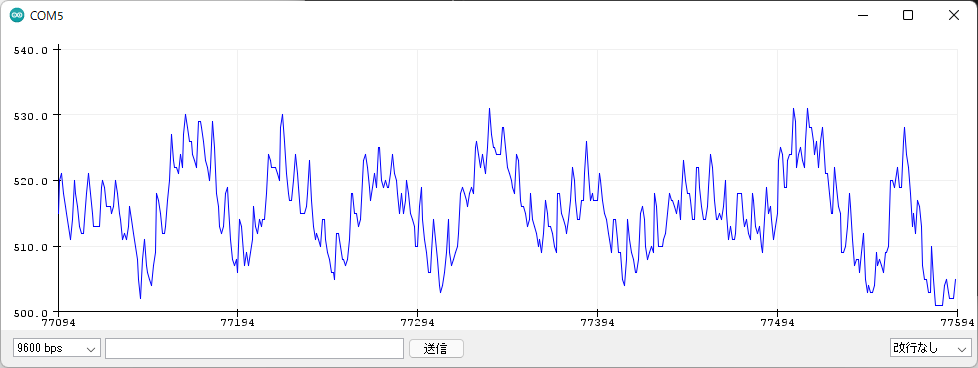
\includegraphics[width=1\textwidth]{2.png}
%     \caption{生成した波形}
%   \end{center}
% \end{figure*}



\begin{multicols}{2}
  \section{今週のアイデア}
  \begin{itemize}
    \item 電話しているときに,インカメラを使って生体情報取得してなんやらする
  \end{itemize}

  \section{先週までのキープ案}
  \begin{itemize}
    \item 手に装着しているスマートウォッチを振動させ,骨密度や筋力の違いによる加速度の変化差分での認証
    \item \sout{ペットボトルの口の部分でパッシブ音響\\センシングし,入水量識別}
    \item シャワーの水量を制御するために,頭皮が濡れている状態だと錯覚させる手法
    \item 歯磨きの磨けてる場所推定
    \item 喉元を使った何か
    \item ぼーっとしている状態の検出と刺激
    \item 歯ぎしり検知
    \item 起立時の行動特徴からその後の行動推定
    \item 乗り物乗車時の加速度センサのキャリブレーション
    \item 足の筋電から歩幅推定
    \item 歯の裏トラックパッド
  \end{itemize}


  \section{ボツ案}
  \begin{itemize}
    \item 視線情報からのマイノリティ検出
    \item 運転中にキョロキョロする回数が少ないと警告
    \item 運動強度の可視化
    \item ジョギング時のペース管理
    \item マウスの掌握やキーボードの打鍵の強さ,触れた回数などからコンディションなどの推定
    \item 椅子着座認識
    \item 心電と脈波の時間差から個人識別
    \item 筋電による状態認識
    \item 物理フリックキーボード
    \item プロジェクターのスクリーンをタッチパネル化
    \item 警報音の目的判別
    \item あおり運転に繋がるドライバーの行動変化
    \item ドライバーの疲労度(腕の下がり)
    \item ライダーの疲労度変化(風圧,気温)
    \item グリップ内蔵型スイッチボックス
    \item 次世代型エンジンスタートシステム(ハンドル圧での認証,ドアノブ圧認証)
    \item 次世代型給油停止システム(センサ型)
    \item 人の歩幅を使った何か…疲労度とか?
    \item センサーで眼を観察して動きなどから視力低下限界警告
    \item 1km以上追越車線を走行した場合のアラートと,車線変更可能位置の誘導などの運転支援
    \item 硬筆文字のデジタル化
    \item シャワーヘッドの動作で識別
    \item ドライヤーの動作で識別
    \item コンセントに圧力センサを取り付けて,撃力(?)から誰が差し込んだかを推定
  \end{itemize}
\end{multicols}

\end{document}
